% ===================================================================
%                       PREÁMBULO DEL DOCUMENTO
% ===================================================================
\documentclass[12pt, a4paper]{article}

% --- PAQUETES ESENCIALES ---
\usepackage[utf8]{inputenc}
\usepackage[spanish,es-lcroman]{babel}

% --- PAQUETES PARA CITAS Y BIBLIOGRAFÍA ---
\usepackage{csquotes}
\usepackage[
    backend=biber,
    style=apa,
    sortcites=true,
    maxcitenames=2,
    giveninits=true,
    date=year,
    urldate=long,
    doi=true,
    hyperref=true
]{biblatex}
\addbibresource{referencias.bib}

% --- PAQUETES PARA DISEÑO, FORMATO Y CONTENIDO ---
\usepackage{geometry}
\geometry{a4paper, margin=2.54cm}
\usepackage{fancyhdr}
\usepackage{graphicx}
\usepackage{float}
\usepackage{caption}
\usepackage{enumitem}
\usepackage{setspace}
\usepackage{mathpazo} % Fuente Palatino
\usepackage{xcolor}
\usepackage{listings}

\definecolor{codegreen}{rgb}{0,0.6,0}
\definecolor{codegray}{rgb}{0.5,0.5,0.5}
\definecolor{codepurple}{rgb}{0.58,0,0.82}
\definecolor{backcolour}{rgb}{0.95,0.95,0.92}

\lstdefinestyle{mystyle}{
    backgroundcolor=\color{backcolour},   
    commentstyle=\color{codegreen},
    keywordstyle=\color{magenta},
    numberstyle=\tiny\color{codegray},
    stringstyle=\color{codepurple},
    basicstyle=\ttfamily\footnotesize,
    breakatwhitespace=false,         
    breaklines=true,                 
    captionpos=b,                    
    keepspaces=true,                 
    numbers=left,                    
    numbersep=5pt,                  
    showspaces=false,                
    showstringspaces=false,
    showtabs=false,                  
    tabsize=2,
    frame=single,
    extendedchars=true,
    literate={á}{{\'a}}1 {é}{{\'e}}1 {í}{{\'i}}1 {ó}{{\'o}}1 {ú}{{\'u}}1 {ñ}{{\~n}}1 {Á}{{\'A}}1 {É}{{\'E}}1 {Í}{{\'I}}1 {Ó}{{\'O}}1 {Ú}{{\'U}}1 {Ñ}{{\~N}}1 {¿}{{?`}}1 {¡}{{!`}}1
}

\lstset{style=mystyle}

% --- PAQUETE HYPERREF ---
\usepackage{xurl}
\usepackage{hyperref}

% --- CONFIGURACIONES ---
\hypersetup{
    colorlinks=true,
    linkcolor=blue!50!black,
    citecolor=blue!50!black,
    urlcolor=cyan!50!black,
    pdftitle={Informe de Resultados de Entrevista},
    pdfauthor={Juan David Julio Serrano et al.}
}

\captionsetup{
    format=plain,
    labelfont=bf,
    textfont=normalfont,
    justification=centering
}

% ===================================================================
%                       INICIO DEL DOCUMENTO
% ===================================================================
\begin{document}

% --- PORTADA ---
\begin{titlepage}
    \begin{center}
        \vspace*{0cm}
        
\includegraphics[width=0.25\textwidth]{../../assets/logo_sena.jpg}
        \vspace*{0.5cm}
        
        {\Huge \bfseries Informe de Aplicación del Instrumento de Recolección de Requisitos para un Sistema de Gemelo Digital de Mantenimiento}\\[2cm]
        
        {\large \bfseries Aprendices:}\\[0.5cm]
        \large{Juan David Julio Serrano (Ficha: 3336237)}\\[0.2cm]
        \large{María Juliana Calvo Corredor (Ficha: 3336237)}\\[0.2cm]
        \large{Jesús David Algeciras Abril (Ficha: 3336238)}\\[0.2cm]
        \large{Didier Moreno Caicedo (Ficha: 3336238)}\\[1.0cm]
        
        {\large \bfseries Instructor:}\\[0.5cm]
        \large{Ing. Wilson Alberto Mosquera Caicedo}\\[1.5cm]
        
        \vspace{1cm}
        \large{Servicio Nacional de Aprendizaje (SENA)}\\[0.3cm]
        \large{Centro de Biotecnología Industrial - Regional Valle}\\[0.3cm]
        \large{Tecnología en Análisis y Desarrollo de Software (ADSO)}\\[1.0cm]
        \large{05 de Diciembre de 2025}
    \end{center}
\end{titlepage}

% --- ÍNDICE ---
\clearpage
\tableofcontents
\clearpage
\doublespacing

% --- CONTENIDO ---

\section{Introducción}

El presente informe documenta la ejecución y los hallazgos obtenidos tras la aplicación del instrumento de recolección de información diseñado para la fase de elicitación de requisitos del proyecto "Sistema de Gemelo Digital para Mantenimiento". Este ejercicio tiene como objetivo validar las hipótesis iniciales sobre las necesidades del sector industrial y descubrir requerimientos funcionales y no funcionales críticos desde la perspectiva de un experto en el dominio.

Para este fin, se utilizó la técnica de la \textbf{entrevista semiestructurada} \parencite{sena:fundamentos2024}, aplicada al Ingeniero Oscar Carrillo, profesional con amplia experiencia en gestión de mantenimiento y confiabilidad en el sector de \textit{Oil \& Gas}. A través de este diálogo, estructurado en bloques temáticos que abarcan desde el diagnóstico del proceso actual hasta la visión futura de la tecnología en planta, se logró recopilar información cualitativa de alto valor estratégico para la definición del producto.

A continuación, se presenta el diseño del instrumento utilizado, la evidencia de su aplicación y un análisis detallado de los resultados, los cuales servirán como base fundamental para la especificación de los requisitos del software a construir.

\section{Diseño del Instrumento (Guion de Entrevista)}

Para la recolección de información, se estructuró una entrevista semiestructurada dividida en cuatro bloques temáticos, diseñada para validar las hipótesis del proyecto y descubrir necesidades no contempladas.

\subsection{Información General (Caracterización del Stakeholder)}

\begin{itemize}
    \item \textbf{Cargo que ocupa actualmente:} \rule{5cm}{0.4pt}
    \item \textbf{Años de experiencia en el área de mantenimiento:} \rule{5cm}{0.4pt}
    \item \textbf{Tipo de industria donde trabaja:} \rule{5cm}{0.4pt}
    \item \textbf{Fecha de la entrevista:} \rule{5cm}{0.4pt}
\end{itemize}

\subsection{Bloque A: Diagnóstico del Proceso Actual y ``Dolores''}

\textit{Este bloque tiene como objetivo mapear el flujo de trabajo actual (``As-Is'') para detectar dependencias manuales, uso de canales informales (llamadas) y puntos de fricción que retrasan la operación.}

\begin{enumerate}
    \item \textbf{Descríbame el proceso completo desde que ocurre una falla hasta que el técnico llega al sitio. ¿Qué pasos intermedios existen?}
    \begin{itemize}
        \item \textit{(Objetivo: Mapear el flujo actual ``As-Is'' y detectar si es excesivamente manual o dependiente de llamadas telefónicas).}
    \end{itemize}
    \item \textbf{¿Cómo registran sus técnicos el trabajo en campo y qué dificultades han reportado con ese método?}
    \begin{itemize}
        \item \textit{(Objetivo: Identificar puntos de fricción en la captura de datos y validar la necesidad crítica de una App móvil).}
    \end{itemize}
    \item \textbf{En su experiencia, ¿cuáles son los principales ``cuellos de botella'' administrativos u operativos que retrasan una reparación urgente?}
    \begin{itemize}
        \item \textit{(Objetivo: Detectar obstáculos externos al técnico, como falta de repuestos o acceso a información, que el sistema debe resolver).}
    \end{itemize}
\end{enumerate}

\subsection{Bloque B: Gestión de la Información y Activos}

\textit{Las siguientes preguntas buscan evaluar la madurez digital de la organización. El propósito es justificar la necesidad de un repositorio documental centralizado y validar la importancia de la trazabilidad histórica en el nuevo sistema.}

\begin{enumerate}
    \item \textbf{¿Cómo es el proceso actual para que un técnico acceda a planos, manuales o historiales en medio de una reparación en campo?}
    \begin{itemize}
        \item \textit{(Objetivo: Justificar la necesidad de un repositorio documental centralizado y vinculado al activo).}
    \end{itemize}
    \item \textbf{¿De qué manera mantienen actualizado el inventario de activos y componentes críticos hoy en día? ¿Es un proceso manual o automático?}
    \begin{itemize}
        \item \textit{(Objetivo: Evaluar la madurez digital actual —Excel vs. Software— para definir el punto de partida del módulo de Activos).}
    \end{itemize}
    \item \textbf{Si necesitáramos ver el historial de fallas de una bomba específica del último año, ¿qué pasos tendría que seguir hoy para obtenerlo?}
    \begin{itemize}
        \item \textit{(Objetivo: Validar la necesidad de trazabilidad histórica y acceso rápido a la "Hoja de Vida" del equipo).}
    \end{itemize}
\end{enumerate}

\subsection{Bloque C: Visión y Toma de Decisiones (KPIs)}

\textit{Este segmento se enfoca en el valor del negocio. Se busca identificar qué métricas (KPIs) deben automatizarse en el Dashboard y validar la propuesta de valor central del Gemelo Digital: la visualización y el monitoreo remoto.}

\begin{enumerate}
    \item \textbf{¿Qué indicadores (KPIs) son prioritarios para su gestión y qué datos específicos debe reunir hoy manualmente para poder calcularlos?}
    \begin{itemize}
        \item \textit{(Objetivo: Identificar qué métricas automatizar en el Dashboard para ahorrar tiempo administrativo).}
    \end{itemize}
    \item \textbf{Describa el procedimiento actual para solicitar un repuesto crítico cuando detectan que el stock está bajo.}
    \begin{itemize}
        \item \textit{(Objetivo: Entender la interacción entre Mantenimiento e Inventario para diseñar el flujo de solicitudes).}
    \end{itemize}
    \item \textbf{¿Qué información crítica de la planta le gustaría visualizar desde su oficina en tiempo real y que hoy no tiene disponible?}
    \begin{itemize}
        \item \textit{(Objetivo: Validar la propuesta de valor central del Gemelo Digital: visibilidad y monitoreo remoto).}
    \end{itemize}
\end{enumerate}

\subsection{Bloque D: Cierre y Visión Futura}

\textit{Finalmente, se utiliza una pregunta abierta para descubrir requisitos deseables o innovadores que no hayan sido contemplados en el alcance inicial.}

\begin{enumerate}
    \item \textbf{Si pudiera diseñar la herramienta ideal para su equipo, ¿qué funcionalidad específica no podría faltar para facilitarles el día a día?}
    \begin{itemize}
        \item \textit{(Objetivo: Pregunta abierta para descubrir ``requisitos deseables'' o innovadores que no hemos considerado).}
    \end{itemize}
\end{enumerate}

\section{Evidencia de Aplicación del Instrumento}

La entrevista se llevó a cabo el día \textbf{02 de diciembre de 2025} mediante la plataforma de videoconferencia Google Meet, con una duración aproximada de \textbf{20 minutos}.

A continuación, se presenta el registro fotográfico de la sesión como evidencia de la ejecución del instrumento con el experto temático.

\begin{figure}[H]
    \centering
    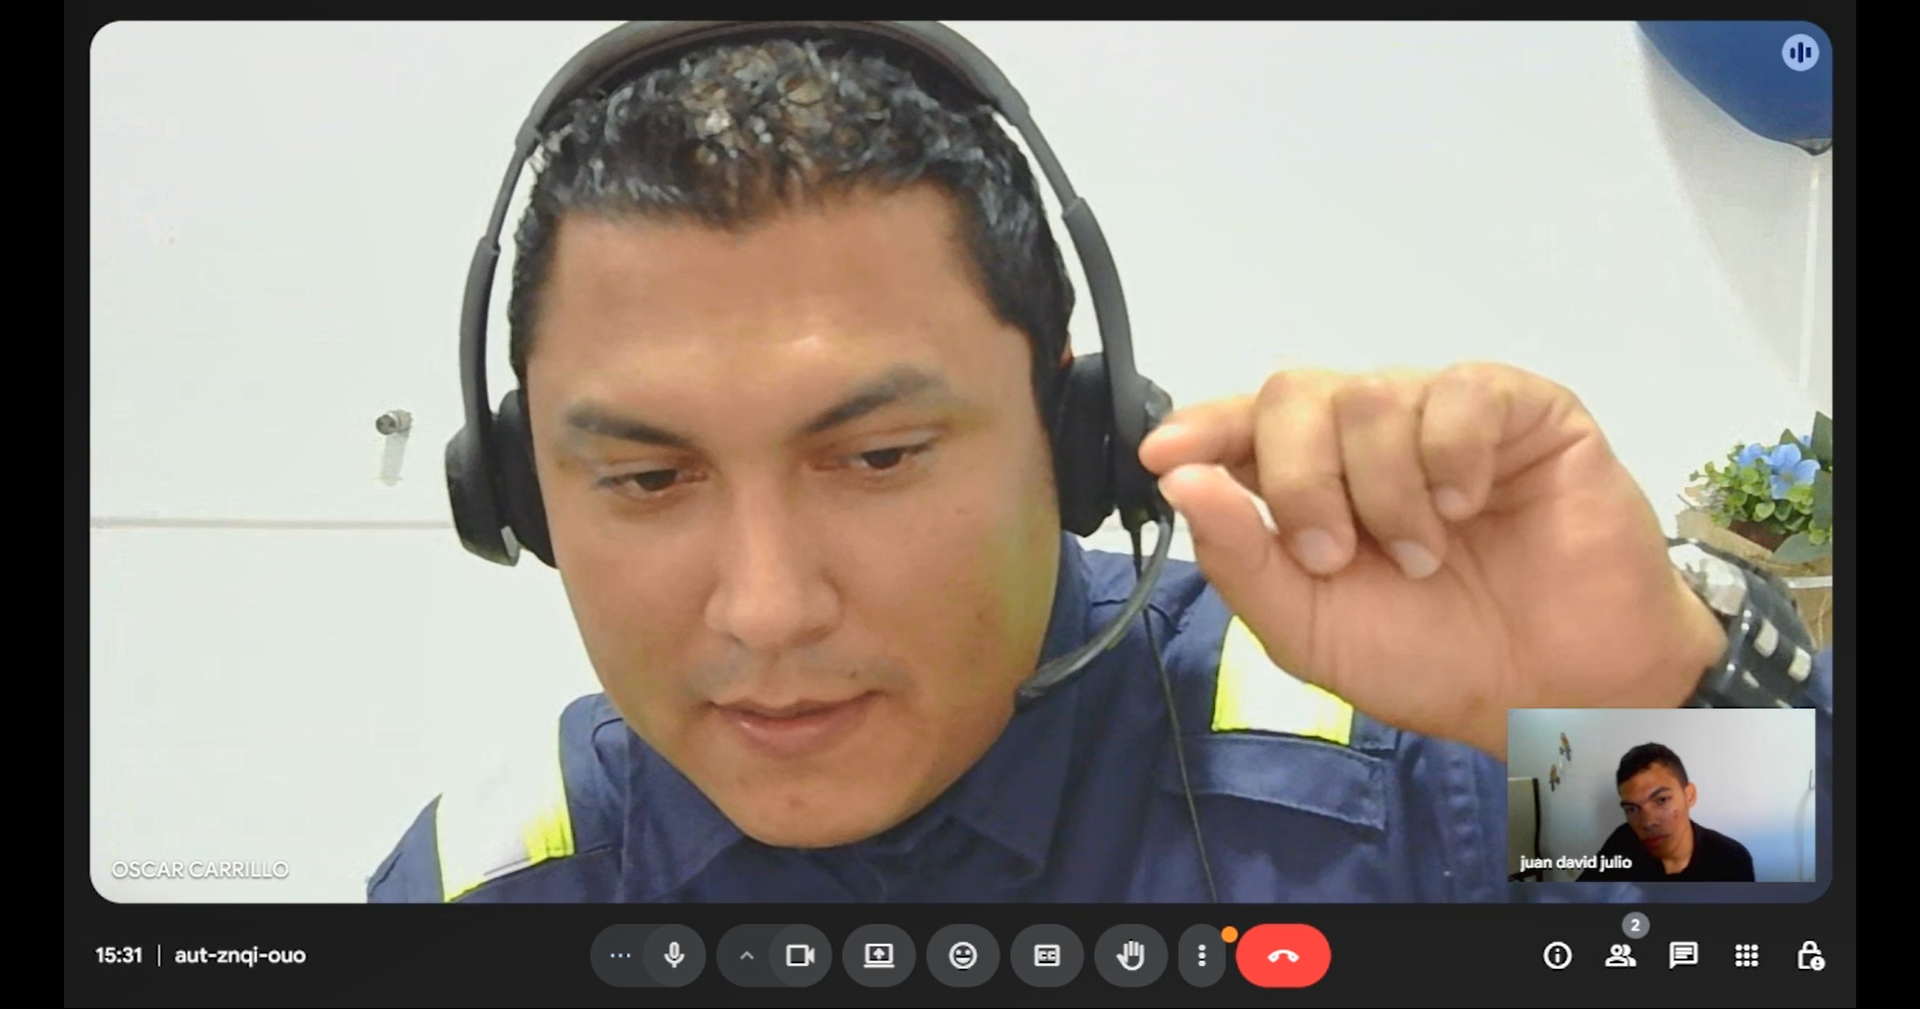
\includegraphics[width=0.8\textwidth]{Imagenes/Evidencia_Entrevista.png}
    \caption{Sesión de validación de requerimientos con el Ing. Oscar Carrillo.}
    \label{fig:evidencia}
\end{figure}

\begin{quote}
Nota: La transcripción completa y depurada de la entrevista se encuentra disponible como anexo al final de este documento.
\end{quote}

\section{Análisis de Resultados}

A partir de la información recolectada con el Ing. Oscar Carrillo (\textbf{Project \& Maintenance Engineer} en el sector Oil \& Gas), se han sintetizado los siguientes hallazgos críticos que validan y refinan los requerimientos del sistema:

\subsection{Diagnóstico del Proceso Actual (Dolores)}

\begin{itemize}
    \item \textbf{Gestión Documental como Cuello de Botella:} Se identificó que, aunque el flujo de trabajo es claro (Solicitud $\rightarrow$ Orden $\rightarrow$ Ejecución), la carga administrativa manual es el principal obstáculo. La generación de órdenes y la transcripción de informes consumen tiempo valioso del personal calificado.
    \item \textbf{Desconexión de Contratistas:} Los reportes digitales de terceros no se integran automáticamente. Existe un ``interfaz humano'' (el Planeador) que debe leer y transcribir datos al sistema central (Infor EAM), lo que valida la oportunidad de automatizar la ingesta de datos mediante IA.
\end{itemize}

\subsection{Gestión de Información y Activos}

\begin{itemize}
    \item \textbf{Acceso a la Información en Campo:} Se confirmó que la información técnica está centralizada pero no es accesible en el sitio de trabajo (``el técnico debe volver al escritorio''). Esto valida la necesidad de una solución móvil que elimine desplazamientos innecesarios.
    \item \textbf{Integridad de Datos (ISO 14224):} La organización sigue estándares rigurosos de taxonomía alineados con los principios de gestión de información de la norma ISO 55001 \parencite{iso:55001}. Esto impone el requisito de que el nuevo sistema debe soportar una estructura jerárquica profunda de activos (hasta nivel de componente) para permitir análisis de causa raíz efectivos.
\end{itemize}

\subsection{Visión y Toma de Decisiones}

\begin{itemize}
    \item \textbf{La Realidad de los KPIs:} Aunque los sistemas actuales pueden calcular métricas como MTBF/MTTR, su fiabilidad depende totalmente de la calidad de la captura de datos en campo. Si el técnico no reporta los datos con precisión, el indicador pierde validez. Por lo tanto, el problema tecnológico a resolver es la \textbf{eficiencia y precisión en la captura de datos}, más que el cálculo en sí mismo.
    \item \textbf{Gestión de Inventario Crítico:} Se validó que el sistema debe gestionar alertas sobre niveles mínimos de ``repuestos de emergencia'', dada la imposibilidad de mantener un stock completo por costos.
    \item \textbf{Validación del Concepto Visual:} El experto confirmó el valor del \textbf{Gemelo Digital 3D}, destacando su utilidad para flexibilizar el trabajo de ingeniería y modernizar la gestión, calificándolo como una herramienta ``bastante interesante y muy práctica''.
\end{itemize}

\subsection{Requerimientos de Innovación}

\begin{itemize}
    \item \textbf{Asistente de Optimización (PMO):} Se detectó una necesidad no contemplada inicialmente: un sistema que no solo registre, sino que \textbf{analice tendencias}. El experto sugiere la implementación de una herramienta analítica que recomiende proactivamente ajustes a los planes de mantenimiento (ej. detección de sobre-mantenimiento), basándose en el análisis histórico de la salud de los activos.
\end{itemize}

\section{Conclusiones}

La aplicación del instrumento ha permitido validar la hipótesis central del proyecto: la pertinencia de un \textbf{Gemelo Digital} no solo como herramienta de visualización, sino como un facilitador crítico para el acceso a la información en campo, resolviendo el problema de los desplazamientos innecesarios y la fragmentación documental.

Adicionalmente, el ejercicio de elicitación ha revelado un requisito de alto valor añadido: la necesidad de integrar \textbf{Inteligencia de Negocios aplicada a la optimización de planes de mantenimiento (PMO)}. Esto sugiere que el sistema debe evolucionar de ser un simple registro pasivo a actuar como un ``asesor inteligente'' que recomienda ajustes basados en el comportamiento real de los activos, alineándose con las tendencias de la Industria 4.0.

% --- BIBLIOGRAFÍA ---
\clearpage
\printbibliography[heading=bibintoc,title=Referencias]

% --- ANEXOS ---
\clearpage
\appendix
\section{Anexo: Transcripción de la Entrevista}

\begin{lstlisting}[language=TeX, caption={Transcripción Entrevista - 02 Dic 2024}]
Fecha: 02 de diciembre de 2024
Participantes:
- Juan David (Entrevistador)
- Ingeniero (Entrevistado - Gerente/Ingeniero de Mantenimiento y Proyectos)

[INICIO DE LA GRABACION]

Juan David:
Ya estamos. Le comento las preguntas para no hacerlo perder tiempo. Primero, quiero confirmar: su cargo es Ingeniero de Mantenimiento y Proyectos, y el sector en el que está actualmente se puede catalogar como Oil & Gas y almacenamiento, ¿cierto?

Ingeniero:
Así es.

Juan David:
La primera pregunta está relacionada con diagnosticar el proceso actual de cómo manejan el mantenimiento y los principales dolores. Quiero que describa el flujo ideal versus el real desde que un operador detecta una falla hasta que el técnico llega al sitio. Es decir, se dañó algún equipo de la planta y se debe comunicar ese fallo hasta el punto donde el técnico llega a planta. Describa los procesos intermedios. Por ejemplo, ¿dónde se pierde más tiempo o información en ese flujo?

Ingeniero:
Mira, todos los activos de la terminal están en el software Infor EAM. ¿Cómo funcionamos? Cuando un equipo presenta una falla o avería, operaciones hace un reporte formal y se genera una orden de trabajo o un requerimiento para el área de mantenimiento. Todo activo tiene su hoja de vida y trazabilidad. Dependiendo de las fallas y de las órdenes que conlleve la reparación, se genera la solicitud; a eso se le hace una orden de trabajo y tenemos un tiempo de respuesta.

Para eso, dependiendo de la empresa, hay un criterio de criticidad. Se define la criticidad del equipo. Puede ser una urgencia, o que se pueda esperar una semana, un mes, o que no sea crítico. Eso se consigna en la solicitud y llega a la plataforma. Tenemos un Planner (Planner y Programador) que revisa la actividad y, desde ahí, delegamos la reparación. Todo esto tiene una línea de tiempo; la idea es que sea rápido, porque dependiendo del equipo hay que dar una solución pronta para no afectar la disponibilidad en la operación.

Juan David:
Listo. Segunda pregunta, relacionada con contratistas externos: cuando se cierra una orden de trabajo, ¿cómo registran hoy el cierre de las órdenes? ¿Usan papel, tablets o lo completan al final del turno?

Ingeniero:
Todo equipo tiene una taxonomía y una frecuencia de mantenimiento establecida. Por ejemplo, una bomba en la terminal tiene dos tipos de mantenimiento. Infor EAM nos avisa: "Para tal fecha está programada la actividad de mantenimiento tipo A o tipo B". Programamos al proveedor; él viene y ejecuta. Generamos el permiso. Al terminar, el proveedor genera un reporte en su formato y nos lo envía digital. Luego, el Planner toma la información, la sube a la carpeta, revisamos el reporte y después lo subimos al sistema. Todo esto es manual: hay una persona que hace esa "interfaz", busca el número de la orden y la sube a Infor EAM.

Juan David:
Tercera pregunta. Desde su rol de supervisor, ¿cuál es el mayor cuello de botella administrativo que impide cerrar una reparación urgente lo más rápido posible? Por ejemplo, permisos de trabajo o recolección de firmas.

Ingeniero:
Para quienes están en supervisión e ingeniería, siempre hay un tema documental que consume tiempo y desgasta el proceso, dependiendo de cómo lo maneje cada empresa. Hay que generar documentación: crear la orden, luego el requerimiento, la orden de compra, después el informe, revisarlo y subirlo al sistema. Eso implica tiempo y, si algún paso no se cumple, se pierde información y la orden queda incompleta, generando reprocesos. La ejecución es rápida; solucionas la bomba. Luego queda la parte documental para mantener la trazabilidad y permitir el análisis de información a futuro, para que el equipo no repita la falla. Es importante, pero termina siendo el cuello de botella.

Juan David:
Cuando un técnico está frente a una bomba o a un equipo y necesita revisar el plano o el manual del fabricante en campo, ¿qué tan fácil es acceder a esa información? ¿La tiene físicamente, de forma digital, o debe volver a la oficina?

Ingeniero:
Depende de cómo esté establecida la taxonomía de equipos y la digitalización de la información. Si estás en campo y requieres información, en muchas empresas está en documentos, en un PC, en un Drive, o en Infor EAM; pero en sitio no siempre se puede revisar. En algunas empresas hay tablets con comunicación directa a Infor EAM, para revisar en tiempo real, pero son pocas. Es algo más de Industria 4.0. La mayoría maneja la información centralizada en PCs o en la nube y hay que ir al escritorio a revisar, lo que implica tiempos de ida y vuelta.

Juan David:
¿Cree que la tendencia es tener esa información menos centralizada en el PC y más disponible de forma multiplataforma (por ejemplo, en una tablet en campo)?

Ingeniero:
Sí. La idea es ahorrar tiempo. Hay cuellos de botella por desplazamientos para consultar información. En algunas empresas ya usan códigos QR en los equipos; el técnico escanea con su tablet y ve la hoja de vida y la información. Pero son pocas por costos y por la madurez de la migración tecnológica. Aún prevalece el mantenimiento preventivo/correctivo tradicional. La tendencia es llegar a esas soluciones.

Juan David:
Usted menciona que implementa ISO 14224 (manejo de datos de falla). ¿Cómo manejan hoy la actualización de la hoja de vida del equipo? Ya explicó el flujo, pero, específicamente, ¿tienen buena integridad de datos históricos para análisis de confiabilidad?

Ingeniero:
La ISO 14224 se enfoca en pilares como la taxonomía de equipos y subequipos: llegar desde el equipo al despiece hasta la última pieza. Tener la data para decir: "En una bomba, tengo la referencia del impeler, la marca, etc.", incluso hasta el tornillo o el motor eléctrico. En la terminal, Infor EAM también se enfoca en la ISO 14224. Subdividimos los equipos hasta el nivel que nos interesa para la data. La idea es crear divisiones para tener más información al hacer análisis causa-raíz, motivos de falla u otras implementaciones de confiabilidad.

Juan David:
Si en un futuro tuvieran un gemelo digital de la planta, ¿le vería valor a acceder en campo a un modelo 3D con despiece de componentes para ubicar partes, saber por dónde comenzar y ver la taxonomía relevante? ¿Sería útil en una aplicación de gemelo digital 3D?

Ingeniero:
Desde 2018 escuché del gemelo digital, especialmente a Rockwell Automation. Tienen una propuesta interesante. Estuve en capacitaciones de gemelo digital y 3D para implementarlo en una planta de proceso, orientado a ver el proceso en tiempo real y a OEE (eficiencia global de equipos), analizando fallas. De ahí a hoy lo he escuchado poco, salvo por tu comentario. Me parece interesante: toda herramienta que flexibilice el trabajo de ingeniería es bienvenida, incluyendo las TIC. Sería práctico.

Juan David:
Para calcular KPI como tiempo medio entre fallas (MTBF) o tiempo medio para reparar (MTTR) en un activo crítico, ¿el sistema lo entrega automáticamente o deben descargar datos a Excel y calcular?

Ingeniero:
Infor EAM tiene opción de analizar MTTR y MTBF y da ese cálculo, siempre y cuando se alimente la información de fallas. Si no se registran los fallos, no puede calcular. Pero la opción existe.

Juan David:
Sobre gestión de repuestos: ¿cómo es la comunicación con el almacén? Según recuerdo, no hay un almacenista como tal en la terminal. ¿Existe un sistema que avise stock para urgencias o debe consultarse con el Planner?

Ingeniero:
No hay un almacén como tal; mantenerlo es costoso. Hemos trabajado en identificar equipos críticos y los repuestos que debemos tener como críticos en la terminal. Por ejemplo, en la báscula hay dos repuestos críticos que debemos tener por si se presenta una falla. Es complejo que una empresa tenga un almacén lleno de repuestos para todo. La clave es el análisis de criticidad para definir repuestos de emergencia. Lo venimos trabajando con el Planner: ya identificamos la báscula, algunos componentes de bombas y otros repuestos de emergencia que debemos tener para resolver contingencias.

Juan David:
Última pregunta, más abierta: si pudiera pedir una funcionalidad "mágica" a un software de mantenimiento que hoy no existe, ¿cuál sería? Algo que realmente usaría y compraría.

Ingeniero:
Estoy alineado con el PMO (plan de optimización de equipos y plan de mantenimiento). Subimos información constantemente; sería interesante que el software sugiriera: "Para el próximo año, mejora con estos equipos". Muchos reportes dicen que "se encuentra bien", y puede haber mantenimientos redundantes que no se requieren. Todo mantenimiento preventivo tiene costo. Buscamos disponibilidad y confiabilidad con ahorro en costos. Esa optimización hoy la hacemos las personas. Ojalá el software lo hiciera y dijera: "En estos activos hay oportunidades de mejora". Luego nosotros validamos y aplicamos. Sería interesante.

Juan David:
Como un asistente para optimización en mantenimiento que da un preliminar y usted lo valida.

Ingeniero:
Exacto.

Juan David:
Eso sería todo por ahora. Muchas gracias por el tiempo. En aproximadamente un año y medio, en fase de ejecución, le muestro el prototipo.

Ingeniero:
Dale, Juan David. Cualquier cosa me avisas. Un gusto saludarte.

Juan David:
Igualmente. Saludos por allá.

Ingeniero:
Igualmente. Chao.

[FIN DE LA GRABACION]
\end{lstlisting}
\end{document}
